\begin{boiboiboite}
	\propeau
	\propair
	\isentropiques
\end{boiboiboite}

\subsubsection{Efficacité d’un moteur}

	Le moteur Diesel d’une excavatrice a une efficacité de~\SI{40}{\percent} et développe une puissance continue de~\SI{80}{ch} (c’est-à-dire \SI{60}{\kilo\watt}). Il est alimenté par du carburant de capacité calorifique \SI{35}{\mega\joule\per\kilogram}.
	
	\begin{enumerate}
		\item Quelle est la consommation horaire de carburant de la machine ?
		\item Quelle est la puissance qu’elle rejette sous forme de chaleur dans le conduit d’échappement ?
	\end{enumerate}

\subsubsection{Efficacité d’un réfrigérateur}

	Un réfrigérateur dont le COP est de~\num{1,2} doit extraire \SI{100}{\kilo\joule} d’un aliment placé dans l’enceinte à basse température. Combien d’énergie électrique consommera-t-il pour cela ? Quelle quantité de chaleur aura-t-il rejeté à la fin du refroidissement ?
	

\subsubsection{Efficacité d’une pompe à chaleur}

	Une pompe à chaleur dont le COP est de~\num{3,1} fournit une puissance de~\SI{4000}{\watt} à une habitation. Quelle est la puissance électrique consommée ? Quelle est la puissance absorbée à l’atmosphère ?

\subsubsection{Thermodynamique de soirée}

	\begin{samepage}
	Un/e étudiant/e assoiffé/e par un cours de thermodynamique interminable prépare son week-end en plaçant un bidon d’eau minérale de~\SI{15}{\liter} (capacité thermique \SI{4,2}{\kilo\joule\per\kilogram\per\kelvin}, \cref{fig_bidon_eau}) au réfrigérateur. Le bidon est à température ambiante (\SI{19}{\degreeCelsius}) et il est ainsi refroidi jusqu’à~\SI{5}{\degreeCelsius}.
	\end{samepage} %handmade
	
	\begin{figure}[htp] %handmade
		\begin{center}
		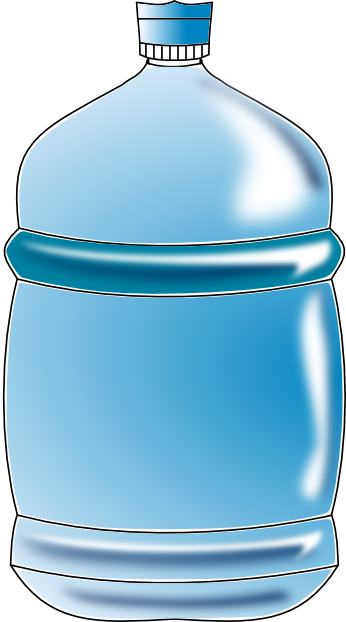
\includegraphics[width=2.5cm]{images/bottle.png}
		\end{center}
		\caption{Ingrédient primaire d’un week-end d’intégration réussi.}
		\label{fig_bidon_eau}
	\end{figure}
	
	
	Le réfrigérateur a un rendement de~\SI{95}{\percent}. Les parois du réfrigérateur, imparfaitement isolées, absorbent de la chaleur de la pièce avec une puissance de~\SI{10}{\watt}.
	
	Au bout de deux heures, la température du bidon a atteint celle de l’intérieur du réfrigérateur.
	
	\begin{enumerate}
		\item Quelle quantité d’énergie électrique le réfrigérateur a-t-il consommée pendant ce temps ?
		\item La pièce s’est-t-elle refroidie, ou réchauffée ?
		\item La pièce se refroidira-t-elle si la porte du réfrigérateur est laissée ouverte ?
	\end{enumerate}


\subsubsection{Pompe à chaleur}

	Décrivez le cycle thermodynamique suivi par le fluide à l’intérieur d’une pompe à chaleur, en indiquant le sens des flux de chaleur et l’emplacement (intérieur/extérieur) des différents composants.
	
	Pourquoi laisse-t-on le fluide se détendre dans une soupape, au lieu d’utiliser une turbine qui pourrait fournir du travail ?
	
	{\small\textit{Cet exercice peut être reproduit en remplaçant «~pompe à chaleur~» par «~climatiseur~», «~réfrigérateur~», ou «~moteur~»}}

\subsubsection{Algèbre}

	Montrez, à partir de la définition du rendement du climatiseur, que celui-ci peut s’exprimer selon la relation :
			\begin{equation}
				\eta_\text{climatiseur} = \frac{1}{\left| \frac{\dot{Q}_\text{out}}{\dot{Q}_\text{in}} \right| - 1} \tag{\ref{rendement_réfrigérateur_qin_qout}}
			\end{equation}
	{\small\textit{Cet exercice peut être reproduit en s’attaquant de la même manière aux équations~\ref{eq_rendement_moteur_qin_qout} et~\ref{eq_rendement_thermopompe_qin_qout}. Attention aux valeurs absolues !}}
	
	
\subsubsection{Refroidissement d’une soufflerie}

	La soufflerie ETW (pour \textit{European Transonic Windtunnel}) permet la circulation d’azote dans un circuit fermé pour observer les écoulements autour de maquettes. Elle permet d’atteindre Mach~\num{0,8} à~\SI{4}{\bar} et~\SI{-200}{\celsius}, à l’aide d’une soufflante de~\SI{50}{\mega\watt}.
	
	Les parois de la soufflerie sont fortement isolées, de sorte que ses transferts thermiques avec l’extérieur sont négligeables devant les autres transferts énergétiques. Le système de refroidissement de l’azote a un COP de~\num{0,8}. 
	
	Lorsque la soufflerie fonctionne à plein régime, quelle puissance mécanique est consommée par le système de refroidissement ? Quelle puissance est rejetée sous forme de chaleur dans l’atmosphère ?


\subsubsection{Génératrice d’électricité à turbine}

	Un turbomoteur est configuré en génératrice de courant électrique (\cref{fig_exo_turbomoteur}) ; il fonctionne avec de l’air atmosphérique.
	
	\begin{figure}
		\begin{center}
		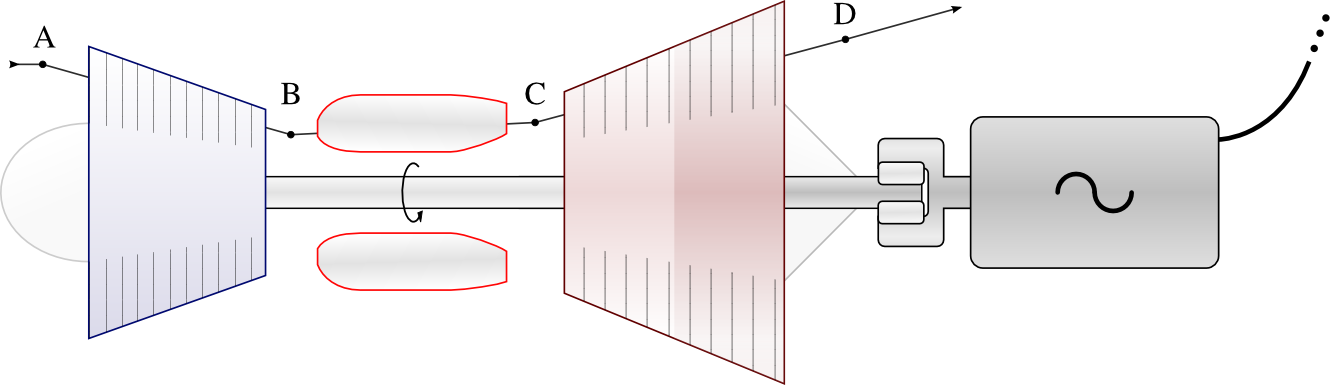
\includegraphics[width=\textwidth]{images/elgen.png}
		\end{center}
		\supercaption{Turbomoteur alimentant une génératrice électrique. On tente généralement de détendre le gaz (dans la turbine, entre C et D) jusqu’à pression atmosphérique.}{schéma \cczero \oc}
		\label{fig_exo_turbomoteur}
	\end{figure}
		
	\begin{itemize}
		\item L’air pénètre dans la machine à~\SI{20}{\degreeCelsius} et~\SI{1}{\bar} avec un débit de~\SI{0,5}{\kilogram\per\second} ; il est comprimé ($\A \to \B$) jusqu’à~\SI{30}{\bar} dans le compresseur.	
		\item L’air reçoit ensuite de la chaleur par combustion, à pression constante ($B \to C$), jusqu’à ce que sa température atteigne \SI{1000}{\degreeCelsius}.	
		\item L’air est enfin détendu dans une turbine ($\C \to D$) jusqu’à retrouver la pression atmosphérique et être rejeté à l’extérieur.
	\end{itemize}
	
	Le compresseur est alimenté mécaniquement par la turbine ; et l’arbre qui les relie entraîne également la génératrice de courant.
	
	Pour étudier le rendement maximal qui pourrait être atteint par la machine, nous considérons que le compresseur et la turbine sont adiabatiques réversibles (c’est-à-dire que la compression et la détente se font de façon très lente et sans transfert de chaleur).

	\begin{enumerate}
		\item À quelle température l’air sort-il du compresseur ?
		\item Quelle est la puissance du compresseur ? Est-ce une puissance fournie ou une puissance consommée ?
		\item À quelle température l’air est-il rejeté dans l’atmosphère ? Quelle puissance est rejetée sous forme de chaleur dans l’atmosphère ?
		\item Quelle est l’efficacité de la machine ?
		\item Comment les quatre transferts énergétiques de cette machine théorique se comparent-ils à ceux d’une machine réelle, dans laquelle le compresseur et la turbine ne peuvent pas être réversibles ?
	\end{enumerate}
	

\subsubsection{Réfrigération industrielle}

	Une chaîne de supermarchés fait appel à votre expertise pour évaluer la rentabilité d’un projet de remplacement de système de réfrigération. 
	
	Tous les supermarchés de l’entreprise utilisent le même modèle de réfrigérateur. Son efficacité est de~\SI{100}{\percent}.
	
	En vous déplaçant jusqu’à un supermarché représentatif, vous effectuez des mesures et étudiez les transferts thermiques du bâtiment, et découvrez que :
	
	\begin{itemize}
		\item La puissance absorbée sous forme de chaleur par la chambre froide des réfrigérateurs, moyennée sur l’année, est de~\SI{80}{\kilo\watt}.
		\item L’hiver, le bâtiment perd de la chaleur avec une puissance moyenne de~\SI{400}{\kilo\watt}. Il est réchauffé avec une batterie de pompes à chaleur de COP \num{4}.
		\item L’été, le bâtiment absorbe de la chaleur avec une puissance moyenne de~\SI{160}{\kilo\watt}. Il est refroidi avec une batterie de climatiseurs de COP \num{0,9}.
		\item Pendant l’automne et le printemps, les besoins en chauffage/refroidissement sont quasi-nuls.
	\end{itemize}
	
	L’entreprise envisage de remplacer toute sa flotte de réfrigérateurs avec un modèle d’efficacité \SI{120}{\percent}, ce qui demande un investissement important. Elle compte 100 supermarchés au total, et paie l’électricité \SI{0,15}{\euroo} par \si{\kilo\watt\hour} en moyenne.
	
	Quelle serait l’économie financière annuelle générée par le changement de réfrigérateur ?
	
\subsubsection{Fonctionnement d’un climatiseur}

	Un climatiseur fonctionne selon le circuit schématisé en \cref{fig_exo_climatiseur}. Le fluide utilisé dans le circuit est de l’air\footnote{On utilise souvent, en pratique, des fluides qui se liquéfient et s’évaporent dans la machine ; mais le principe de fonctionnement reste le même.}\nolinebreak.
	
	\begin{figure}
		\begin{center}
		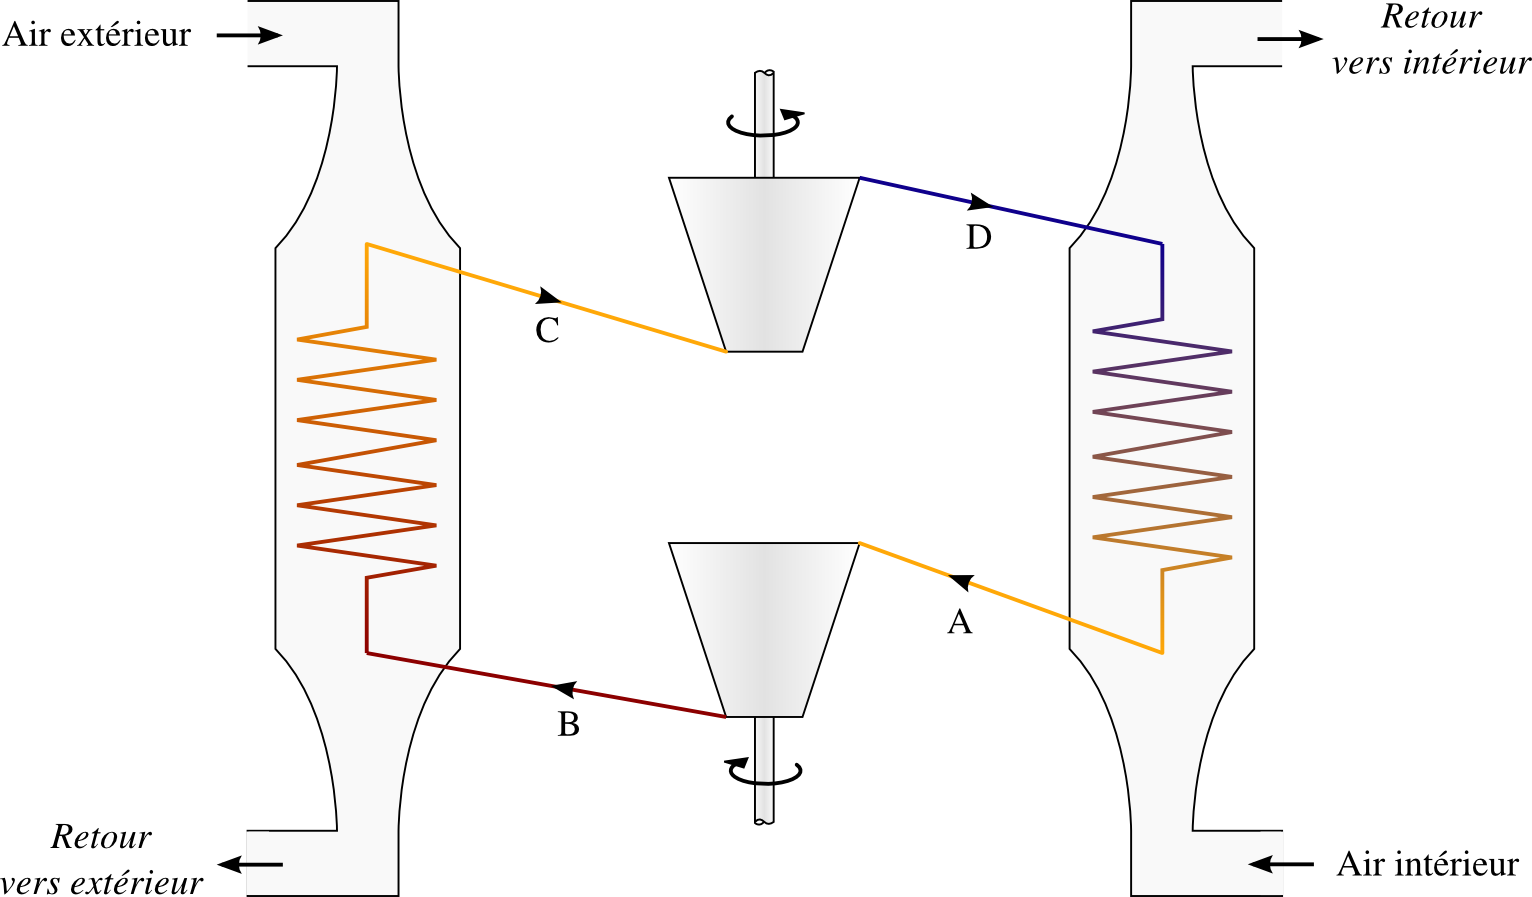
\includegraphics[width=\textwidth]{images/aircon_pack.png}
		\end{center}
		\supercaption{Schéma de principe d’un climatiseur. L’air du circuit du climatiseur tourne en continu ($\A \to \B \to \C \to D \to A$), sans jamais quitter la machine.}{schéma \cczero \oc}
		\label{fig_exo_climatiseur}
	\end{figure}
	
	L’air à l’intérieur du circuit y tourne de façon continue. Le compresseur et la turbine sont tous les deux adiabatiques et nous considérons qu’ils sont réversibles. Les échanges de chaleur se font à pression constante.

	Lorsqu’on met en route le climatiseur, la température extérieure et la température intérieure sont égales à~\SI{30}{\degreeCelsius}.
 
	Les températures de l’air à l’intérieur du circuit sont $T_\A = \SI{20}{\degreeCelsius}$, $T_\B = \SI{60}{\degreeCelsius}$, et $T_\C = \SI{40}{\degreeCelsius}$.

	\begin{enumerate}
		\item Représentez l’évolution de l’air du circuit sur un diagramme pression-volume, en y représentant les transferts de travail et de chaleur.
		\item Quel est le rapport des pressions entre A et B ?
		\item Quelle est la température de l’air du circuit en D ?
		\item Calculez les puissances spécifiques pour chacun des quatre transferts énergétiques, et calculez ainsi l’efficacité du climatiseur.
		\item Le/la propriétaire souhaite obtenir un flux d’air frais à~\SI{10}{\degreeCelsius} de débit \SI{0,25}{\metre\cubed\per\second}. Quelle puissance électrique faut-il fournir au climatiseur pour cela ?
		\item Quel sera alors le débit minimal d’air extérieur à faire circuler dans la section extérieure du climatiseur ?
		\item Pendant l’hiver, le/la propriétaire souhaite modifier le climatiseur pour le transformer en pompe à chaleur. Décrivez (qualitativement) une modification du circuit pour cela, et tracez l’évolution de l’air du circuit sur un nouveau diagramme pression-volume en y indiquant les transferts énergétiques.
	\end{enumerate}


\subsubsection{Performances d’un réfrigérateur domestique}

	Un/e ingénieur/e fait l’achat d’un réfrigérateur domestique (\cref{fig_exo_refrigerator}) et se surprend de ne pas trouver mention de son efficacité dans le copieux manuel d’utilisation. Il/elle tente de l’estimer à l’aide des caractéristiques indiquées au dos du réfrigérateur :
		
	\begin{figure}
		\begin{center}
		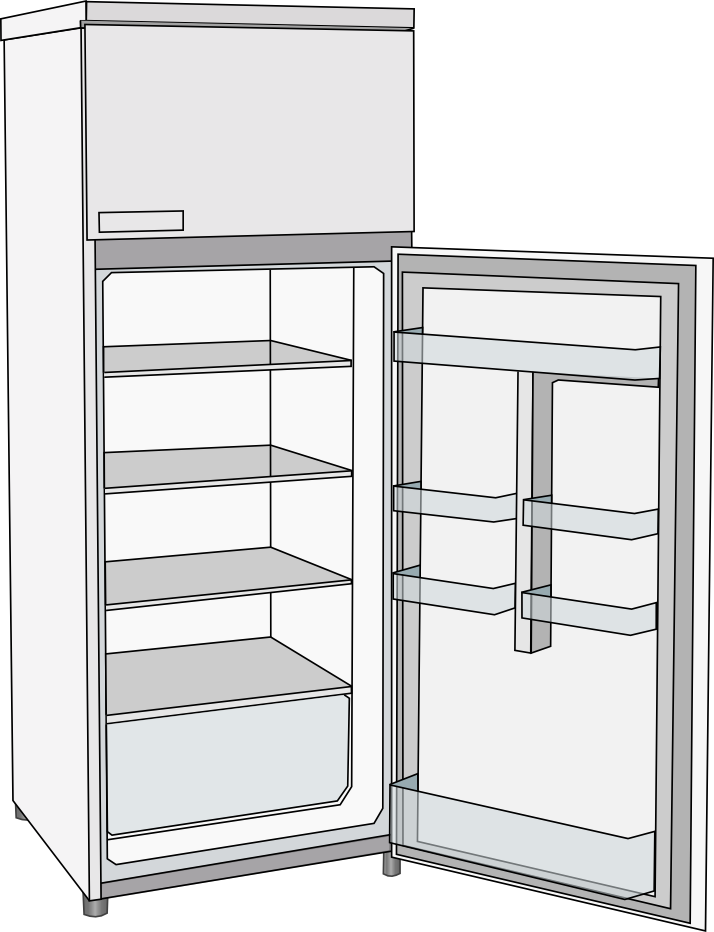
\includegraphics[width=3.5cm]{images/refrigerator.png}
		\end{center}
		\caption{Fascinante machine thermodynamique}
		\label{fig_exo_refrigerator}
	\end{figure}
		
	\begin{itemize}
		\item Puissance \SI{90}{\watt}	(interprétation : puissance électrique maximale)
		\item Consommation \SI{0,548}{kWh/24h}	(interprétation : puissance électrique moyenne)
		\item Capacité de congélation : \SI{2}{kg/24h}.	(interprétation : puissance de congélation maximale, pour de l’eau pure)
		\item Contenance : congélateur \SI{40}{\liter}, réfrigérateur \SI{112}{\liter}
	\end{itemize}
	
	La capacité calorifique massique de l’eau liquide est de~\SI{4,2}{\kilo\joule\per\kilogram\per\kelvin}. Son changement de phase nécessite en outre \SI{300}{\kilo\joule\per\kilogram}. Une fois solide, sa capacité calorifique massique est de~\SI{2,04}{\kilo\joule\per\kilogram\per\kelvin}. 
	
	\begin{enumerate}
		\item Si la puissance maximale de congélation du réfrigérateur est atteinte lorsqu’il fonctionne à puissance maximale, et que l’on néglige les défauts d’isolation, quelle est son efficacité ?
		\item On suppose que la consommation électrique moyenne annoncée (\SI{0,548}{kWh/24h}) est mesurée en mode de fonctionnement normal (toutes températures stabilisées), sans ouvrir la porte. Dans ce cas, quelle est la puissance des pertes de la chambre froide sous forme de chaleur ?
		\item En estimant le volume d’air renouvelé lors de l’ouverture de la porte, calculez le coût électrique d’une brève ouverture de la porte du réfrigérateur.
	\end{enumerate}


\subsubsection{Cycle moteur à vapeur}

	Dans une centrale à vapeur, l’eau circule en continu en traversant quatre composants :
	
	\begin{itemize}
		\item Une pompe quasi-adiabatique dans laquelle elle rentre à l’état de liquide saturé et qui porte sa pression depuis \SI{0,5}{\bar} jusqu’à~\SI{40}{\bar} ;
		\item Une chaudière dans laquelle sa température est portée à~\SI{620}{\degreeCelsius}, à pression constante ;
		\item Une turbine quasi-adiabatique qui laisse l’eau retourner jusqu’à~\SI{0,5}{\bar} en perdant de l’énergie sous forme de travail ;
		\item Un condenseur qui refroidit l’eau à pression constante (\SI{0,5}{\bar}) jusqu’à son retour dans la pompe.
	\end{itemize}
	
	Nous supposons en outre que :
		\begin{itemize}
			\item À la sortie de la turbine, la vapeur est\footnote{Après le \courshuit nous saurons prédire cette température de sortie.} à température de~\SI{110}{\degreeCelsius}.
			\item La pompe est quasi-réversible et que la masse volumique de l’eau ne varie pas lorsqu’elle la traverse.
		\end{itemize}
	
	Quelle est l’efficacité du moteur ?

\subsubsection{Calculs thermodynamiques de cuisine}

	Il est souvent dit qu’il ne faut pas placer d’aliments encore «~chauds~» au réfrigérateur. Le but de cet exercice est d’identifier et de quantifier le surcoût engendré.\nopagebreak %handmade
	
	On place un aliment (\SI{1}{\kilogram}) de capacité thermique \SI{6}{\kilo\joule\per\kilogram\per\kelvin} encore «~chaud~» (température~\SI{30}{\celsius}) au réfrigérateur (\SI{5}{\degreeCelsius}).
	
	\begin{enumerate}
		\item Quelle quantité de chaleur le réfrigérateur devra-t-il lui soutirer pour l’amener à température de conservation ?
		\item Quel est l’excédent par rapport au cas où l’aliment aurait été inséré à température ambiante (\SI{20}{\degreeCelsius}) ?
	\end{enumerate}
	
	Cet excédent énergétique devra être inutilement extrait de la chambre froide par le réfrigérateur, et représente ainsi un coût électrique que l’on souhaite quantifier.
	
	Nous supposons que le réfrigérateur, ancien, a un rendement de~\SI{65}{\percent}, et nous négligeons ses défauts d’isolation, tout comme ceux de la pièce qui le contient.
	
	\begin{enumerate}
		\shift{2}
		\item Quelle quantité supplémentaire d’énergie électrique est consommée par le réfrigérateur ?
		\item Quelle quantité supplémentaire de chaleur est rejetée dans la pièce par le réfrigérateur ?
	\end{enumerate}

	Le tarif d’électricité local est de \SI[per-mode = symbol]{0,15}{\euroo\per\kilo\watt\per\hour}. Quel aura été le coût total engendré par le fait d’avoir placé l’aliment encore «~chaud~» au réfrigérateur :
		
	\begin{enumerate}
	\shift{4}
		\item si la pièce est chauffée avec un radiateur électrique ? \\
			(la chaleur dégagée par le réfrigérateur ne doit alors pas être dégagée par le radiateur)
		\item si la pièce est chauffée avec une thermopompe de COP \num{3,5} ?	\\ 
			(la chaleur dégagée par le réfrigérateur ne doit alors pas être dégagée par la thermopompe)
		\item si la pièce est climatisée à l’aide d’un climatiseur d’efficacité \num{0,8} ?\\
			(la chaleur dégagée par le réfrigérateur devant alors être extraite par le climatiseur)
	\end{enumerate}

\exercisesolutionpage
\titreresultats
	\linktosolutionsblurb

	\begin{description}
		\item [6.1] \tab 1) $\dot{m} = \SI{15,4}{\kilogram\per\hour}$ 
						\tab 2) $\dot{Q}_\text{out} = \SI{-90}{\kilo\watt}$
		\item [6.2] \tab ${W}_\text{net} = \SI{+83,3}{\kilo\joule}$ ; $Q_\text{out} = \SI{-183,3}{\kilo\joule}$
		\item [6.3] \tab $\dot{W}_\text{net} = \SI{+1,29}{\kilo\watt}$ ; $\dot{Q}_\text{in} = \SI{+2,71}{\kilo\watt}$
		\item [6.4]	\tab 1) ${W}_\text{net} = \SI{+1004,2}{\kilo\joule}$
						\tab 2) réchauffée
						\tab 3) non, elle se réchauffera également
		\item [6.7] \tab $\dot{W}_\text{net réf.} = \SI{+62,5}{\mega\watt}$ (sacré réfrigérateur) ; $\dot{Q}_\text{out réf.} = \SI{-112,5}{\mega\watt}$
		\item [6.8] \tab 1) $T_\B = \SI{774,3}{\kelvin}$ 
						\tab 2) $\dot{W}_\fromatob = \SI{+241}{\kilo\watt}$ 
						\tab 3) $T_\D = \SI{581,7}{\kelvin}$ ; $\dot{Q}_\fromdtoa = \SI{-94,8}{\kilo\watt}$ 
						\tab 4) \SI{62,3}{\percent} 
						\tab 5) voir \S\ref{ch_évolutions_irr_sf}
		\item [6.9] \tab Économie annuelle de~\SI{-21,32}{\kilo\euroo} par supermarché. Les nouveaux réfrigérateurs permettent d’économiser \SI{13,3}{\kilo\watt} au printemps/automne, \SI{10,1}{\kilo\watt} en hiver, \SI{28,2}{\kilo\watt} en été.
		\item [6.10] 	\tab 3) $\frac{p_\B }{p_\A} = \num{1,565}$ 
							\tab 4) $T_\D = \SI{275,4}{\kelvin}$ 
							\tab 5) $w_\text{in} = \SI{+40,2}{\kilo\joule\per\kilogram}$ ; $q_\text{out} = \SI{-20,1}{\kilo\joule\per\kilogram}$ ; $w_\text{out} = \SI{+37,79}{\kilo\joule\per\kilogram}$ ; $q_\text{in} = \SI{+17,69}{\kilo\joule\per\kilogram}$ ; $\eta = \num{7,326}$ 
							\tab 6) $\dot{W}_\text{net} = \SI{+845}{\watt}$ ; $\dot{m}_{circuit} = \SI{0,35}{\kilogram\per\second}$
		\item [6.11] 	\tab 1) $\eta = \num{0,101}$ (en pratique plus haut) 
							\tab 2) $\dot{Q}_{parois} = \SI{2,31}{\watt}$ 
							\tab 3) En estimant \SI{56}{\liter} : \SI{0,42}{ct}
		\item [6.12] \tab \SI{31,47}{\percent}
		\item [6.13] 	\tab 1) \SI{150}{\kilo\joule} 
							\tab 2) \SI{60}{\kilo\joule} 
							\tab 3) \SI{92,3}{\kilo\joule} 
							\tab 4) \SI{-152,3}{\kilo\joule} 
							\tab 5) \SI{0}{\joule} 
							\tab 6) \SI{41,53}{\kilo\joule} 
							\tab 7) \SI{282,7}{\kilo\joule} soit un coût effarant de~\SI{0,012}{\euroo}.
	\end{description}
